\documentclass[french]{article}
\usepackage{amsmath}
\usepackage{amssymb}	% packages that allow mathematical formatting
\usepackage{graphicx}	% package that allows you to include graphics
\usepackage{setspace}	% package that allows you to change spacing
\usepackage{fullpage}	% package that specifies normal margins
\usepackage{microtype}
\usepackage{amsthm}
\newcommand{\argmin}{\operatornamewithlimits{argmin}}
\newcommand{\argmax}{\operatornamewithlimits{argmax}}
\usepackage{listings}
\usepackage{color}
\usepackage{caption}
\usepackage{subcaption}
\usepackage{rotating} % Rotating table
\usepackage{enumerate}


\definecolor{codegreen}{rgb}{0,0.6,0}
\definecolor{codegray}{rgb}{0.5,0.5,0.5}
\definecolor{codepurple}{rgb}{0.58,0,0.82}
\definecolor{backcolour}{rgb}{0.95,0.95,0.95}



\lstdefinestyle{mystyle}{
	backgroundcolor=\color{backcolour},   
	commentstyle=\color{codegreen},
	keywordstyle=\color{blue},
	numberstyle=\tiny\color{codegray},
	stringstyle=\color{codepurple},
	basicstyle=\ttfamily\footnotesize,
	breakatwhitespace=false,         
	breaklines=true,                 
	captionpos=b,                    
	keepspaces=true,                 
	numbers=none,                    
	numbersep=5pt,                  
	showspaces=false,                
	showstringspaces=false,
	showtabs=false,                  
	tabsize=2,
	otherkeywords={!,!=,~,*,\&,\%/\%,\%*\%,\%\%,<-,<<-,/}
}\lstset{style=mystyle}

\usepackage[left=2.5cm, right=2.5cm, top=2cm, bottom = 3cm]{geometry}


\lstdefinestyle{mystyle}{
	backgroundcolor=\color{backcolour},   
	commentstyle=\color{codegreen},
	keywordstyle=\color{blue},
	numberstyle=\tiny\color{codegray},
	stringstyle=\color{codepurple},
	basicstyle=\ttfamily\footnotesize,
	breakatwhitespace=false,         
	breaklines=true,                 
	captionpos=b,                    
	keepspaces=true,                 
	numbers=none,                    
	numbersep=5pt,                  
	showspaces=false,                
	showstringspaces=false,
	showtabs=false,                  
	tabsize=2,
	otherkeywords={!,!=,~,*,\&,\%/\%,\%*\%,\%\%,<-,<<-,/}
}\lstset{style=mystyle}


\begin{document}
\noindent Patrick Shultz\\
Mehra and Prescott

\paragraph{1}
The economy consists of a representative agent with preferences:
\begin{equation*}
	U(c) = E_0 \sum_{t=0}^{\infty}\beta^tu(c_t), \quad u(c) = \frac{c^{1-\alpha}}{1-\alpha}
\end{equation*}
There is no production. Aggregate endowment each period follows the stochastic process
\begin{equation*}
	y_{t+1} = \lambda_{t+1}y_t
\end{equation*}
where the growth rate $\lambda$ takes on one of two value, $\lambda_1$ or $\lambda_2$, with probabilities given by the first order Markovian transition matrix:
\begin{equation*}
	\Pi = \begin{bmatrix} 
	(1+\rho)/2 & (1-\rho)/2\\(1-\rho)/2 & (1+\rho)/2
	\end{bmatrix}
	=\begin{bmatrix} 
	\phi & 1-\phi\\1-\phi & \phi
	\end{bmatrix}
\end{equation*}
Let $\lambda_1=\mu + \sigma$, and $\lambda_2 = \mu-\sigma$. In equilibrium $y_t = c_t$. \\

Download Non-durable and service consumption data from WRDS. Generate real-per capita consumption growth for two sample (a) one that starts at 1929, (b) one that starts at 1950. 

\begin{figure}[!htb]
	\centering
	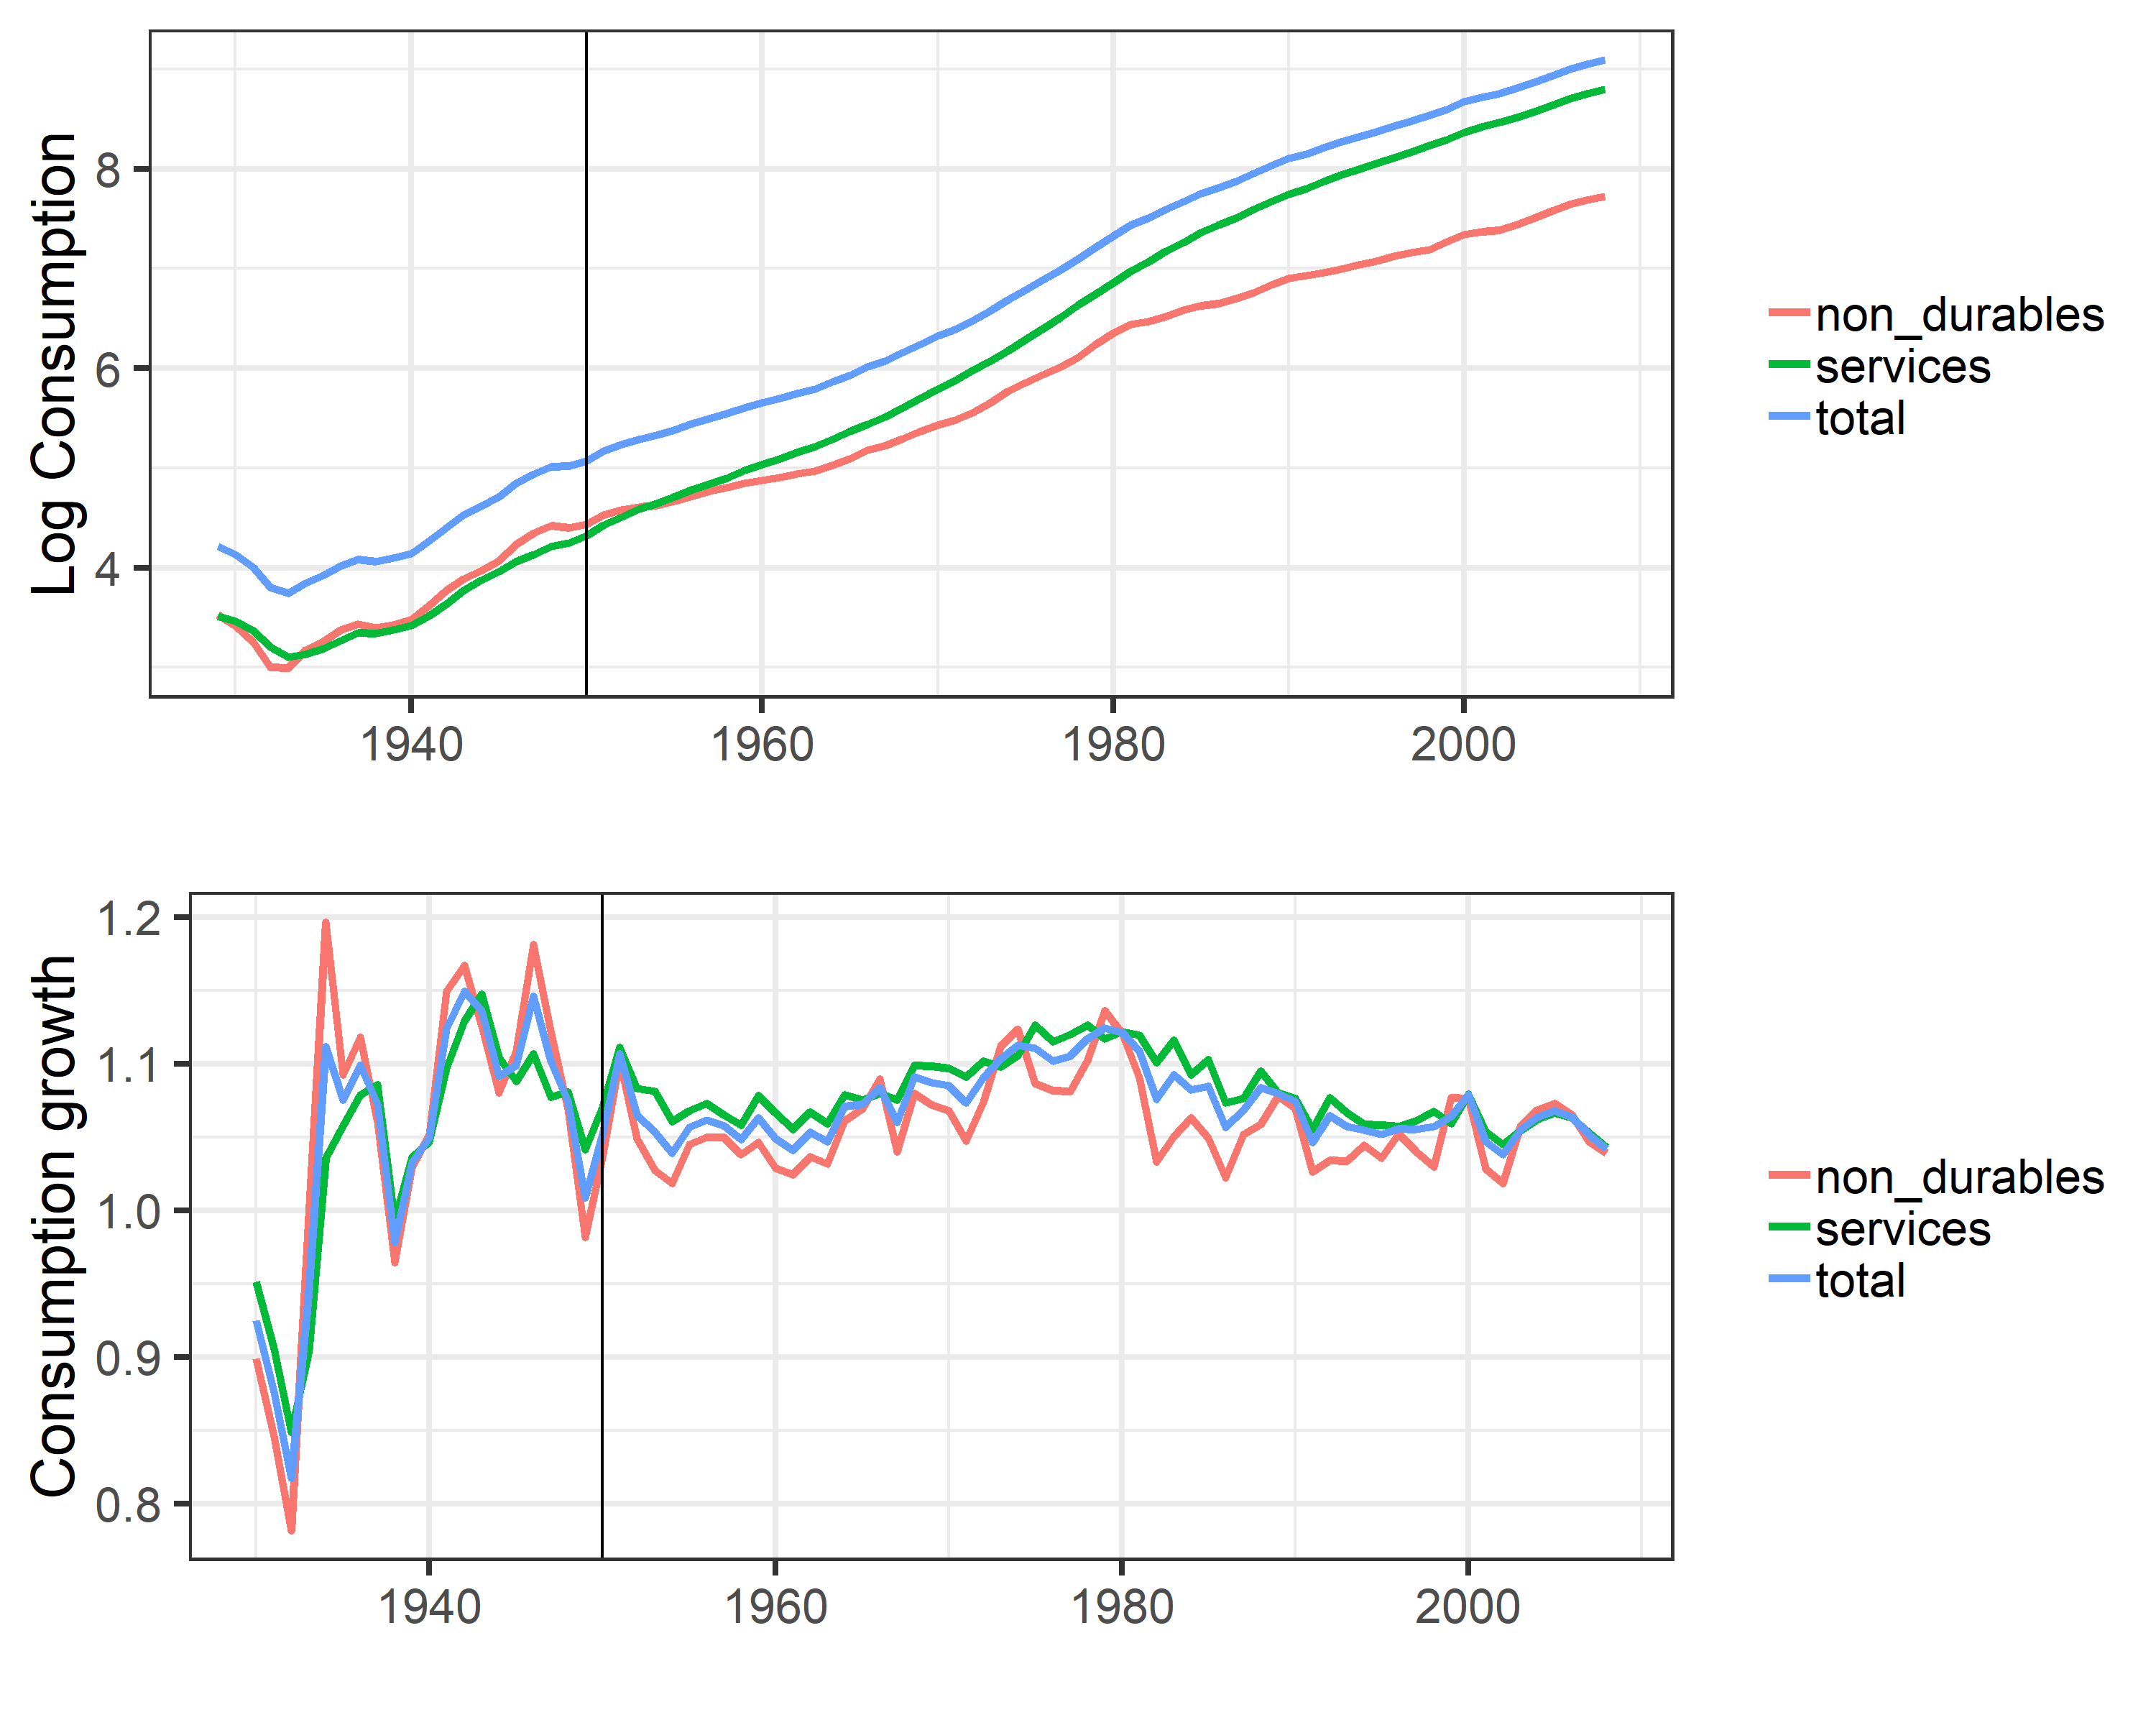
\includegraphics[width=0.75\textwidth]{connsumption_growth.png}
	\label{fig:consumption_data}
	\caption{Log Consumption and Consumption Growth (Gross). Vertical line represents starting point of sample (b)}
\end{figure}

Mehra and Prescott find $0.018$, $0.036$, and $-0.14$, are the mean, standard deviation and autocorrelation of continuous mean consumption growth in their sample, respectively. We can then calculate the parameters of the Markov process as follows:
\begin{itemize}
	\item \textbf{Persistence:} To compute the persistence of the process, consider the indicator function, denoted as  $\xi_t$, which is equal to $1$ in the high growth state and zero otherwise.  Given our transition matrix $\Pi$, we then have 
	\begin{equation*}
	\begin{bmatrix}
	\xi_{t}\\ 1- \xi_t
	\end{bmatrix} = \begin{bmatrix} 
	\phi & 1-\phi\\1-\phi & \phi
	\end{bmatrix} \begin{bmatrix}
	\xi_{t-1}\\ 1- \xi_{t-1}
	\end{bmatrix}
	+
	\begin{bmatrix}
	v_{1, t}\\ v_{2, t}
	\end{bmatrix}
	\end{equation*}
	which implies $\xi_{t+1} = (1-\phi) + \xi_t(\phi -1 +\phi) + v_{1, t+1}$. Taking the unconditional expectation implies the persistence in the process is given by $2\phi -1 = 2(\frac{1}{2}(1+\rho))-1 = \rho$. Thus, $2\phi -1 = -0.014$, and $\phi = 0.43$. Further note that $E\left[\xi_{t+1}\right] = \frac{1-\phi}{2(1-\phi)}$. Thus, the unconditional probability $\pi_1 = \pi_2 = 0.5$. 
	\item\textbf{Mean:} Given that the mean gross growth rates in the high and low growth regimes are given by $\mu + \sigma$ and $\mu -\sigma$, we know that the unconditional mean is given by $\mu = 1.018$.
	\item \textbf{Standard Deviation:} Once again using the unconditional probability derived above, we have that the unconditional variance of the process is given by	$\sigma^2 = 0.5 \sigma^2 + 0.5\sigma^2$, which implies $\sigma = 0.036$. 
\end{itemize}

We can follow the same the process to calculate the parameters for sample (a) and sample (b). \\


%-------------------------------------------------------------------------------
% Markov chain calculations 
%-------------------------------------------------------------------------------


\paragraph{a) Markov Chains}
\begin{enumerate}[I.]
	\item Compute the conditional moments of the Markov chain which describes the evolution of the  $\lambda$ process.\\
	
	 Letting $s_t = h/l$ denote whether we are currently in the high or low state, the conditional means are given by
	\begin{equation*}
		\begin{split}
		E\left[\lambda_{t+1}|s_t = h\right] &= \pi_{hh}\lambda_h + \pi_{hl}\lambda_l \\
		&= \phi(\mu + \sigma) + (1-\phi)(\mu-\sigma)\\
		&= \mu + \sigma(2\phi -1)\\
		E\left[\lambda_{t+1}|s_t = l\right]&=\pi_{lh}\lambda_h + \pi_{ll}\lambda_l \\
		&= (1-\phi)(\mu + \sigma) + \phi(\mu-\sigma)\\
		&= \mu +\sigma(1-2\phi)\\
		\end{split}
	\end{equation*}
	The conditional variance is generally given by 
	\begin{equation*}
	\begin{split}
		Var(\lambda_{t+1}|s_t=i)&=E\left[\lambda_{t+1}^2|s_t = i\right] - E\left[\lambda_{t+1}|s_t = i\right]^2\\
		&= \sum_j \pi_{ij} \lambda_j^2 - \left(\sum_j \pi_{ij}\lambda_j\right)^2
	\end{split}
	\end{equation*}
	Thus, we have 
	\begin{equation*}
	\begin{split}
		Var(\lambda_{t+1}|s_t = h) &= \pi_{hh}\lambda_h^2 + \pi_{hl}\lambda_l^2 - (\pi_{hh}\lambda_h + \pi_{hl}\lambda_l)^2\\
		&= \phi(\mu + \sigma)^2 + (1-\phi)(\mu-\sigma)^2 + (\phi(\mu + \sigma) - (1-\phi)(\mu-\sigma))^2\\
		&= 4 \sigma ^2 \phi(1-\phi) \\
		Var(\lambda_{t+1}|s_t = l) &=\pi_{lh}\lambda_h^2 + \pi_{ll}\lambda_l^2 - (\pi_{lh}\lambda_h + \pi_{ll}\lambda_l)^2\\
		&= 4 \sigma ^2 \phi(1-\phi) 
	\end{split}
	\end{equation*}
	Hence, we see that the conditional variances are equal to each other. 
	\item Compute the stationary distribution $\Pi^*$, which satisfies $\Pi^* = \Pi \times \Pi^*$. \\
	
	We know that $\Pi^*\iota = 1$, where $\iota$ denotes the vector of ones. Using these two restrictions, we can solve for $\Pi^*$. Define the matrix $A$ as 
	\begin{equation*}
		A = \begin{bmatrix}
		I_2 - \Pi \\ \iota'
		\end{bmatrix}
	\end{equation*}
	Then we have $A\Pi^* = \left[0\quad0\quad 1\right]'$. The solution for $\Pi^*$ is 
	\begin{equation*}
	\begin{split}
	A\Pi^* &= \left[0\quad0\quad 1\right]'\\
	A'A\Pi^* &= A'\left[0\quad0\quad 1\right]'\\
	\Pi^* &= (A'A)^{-1}A'\left[0 \quad 0 \quad 1\right]'
	\end{split}
	\end{equation*}
	Plugging in our parameters for $\phi$, we get 
	\begin{equation*}
		\Pi^* =	
		\begin{bmatrix}
		0.5\\ 0.5
		\end{bmatrix}
	\end{equation*}
	\item Confirm that the unconditional mean, standard deviation, and first order autocorrelation coeffcient for the $\lambda$ process are $\mu, \sigma$, and $\rho$ respectively. \\
	
	We can calculate the unconditional mean and standard deviation using $\Pi^*$
	\begin{equation*}
		\begin{split}
		E\left[\lambda\right] &= \sum_i \pi_{i}^*\lambda_i\\
		&= 0.5 (\mu+\sigma) + 0.5(\mu -\sigma)\\
		&= \mu\\
		Var(\lambda)&= \sum_i \pi_{i}^* \lambda_i^2 - \left(\sum_i \pi_{i}^*\lambda_i\right)^2\\
		&=0.5 (\mu+\sigma)^2 + 0.5(\mu -\sigma)^2 - (0.5 (\mu+\sigma) + 0.5(\mu -\sigma))^2\\
		&= 0.5( (\mu+\sigma)^2 +(\mu -\sigma)^2) - \mu^2\\
		&=  0.5( 2(\mu^2+\sigma^2)) - \mu^2\\
		& = \sigma^2
		\end{split}
	\end{equation*}
	Thus, we have verified that the unconditional mean and standard deviation are $\mu$ and $\sigma$, respectively. 
\end{enumerate}


%-------------------------------------------------------------------------------
% Term Structure of Interest Rates 
%-------------------------------------------------------------------------------

\paragraph{b) The Term Structure of Interest Rates:} In this economy, like other real economies, an $n$ period bond is a sure claim to a single unit of risk free consumption $n$ periods hence. 

\begin{enumerate}[I.]
	\item Use the agent's first order condition to compute the price $b^1_i$ and the return $R^1_i$, on a one-period bond in each state $i$. Choose $\beta$ to produce a mean real interest rate of $5$ percent (i.e. $R = 1.05$). \\
	
	Let $i$ denote a state in $\Omega$ (the set of all states) and $q_t(i)$ denote the time $t$ price of an Arrow-Debreu security that pays off in state $i\in\Omega$. Then $b_i^1$ at time $t$ is given by 
	\begin{equation*}
		b_i^1 = \sum_{i\in\Omega}q_t(i) = \sum_{i\in\Omega}\pi_t(i)\beta \frac{u'(c_{t+1})}{u'(c_t)} = \beta E_t\left[\frac{u'(c_{t+1})}{u'(c_t)}\right] = \beta E \left[(c_{t+1}/c_t)^{-\alpha}\right] = \beta E\left[\lambda_{t+1}^{-\alpha}\right]
	\end{equation*}
	where $\lambda_{t+1}$ is the growth rate in consumption from time $t$ to $t+1$. We can use our Markov chain to compute this expectation, so our general expression for the one period bond price in state $i$ is 
	\begin{equation}
	\begin{split}
		b^1_i = \beta \sum_{j=1}^{N}\pi_{ij}\lambda_j^{-\alpha}
	\end{split}
	\label{eq:bond_price}
	\end{equation}
	Thus, when $i = 1$ (the high state), we have the following bond price
	\begin{equation*}
	\begin{split}
			b^1_1 &= \beta \sum_{j=1}^{N}\pi_{1j}\lambda_j^{-\alpha}\\
			&=\beta \left(\pi_{11}\lambda_1^{-\alpha} + \pi_{12}\lambda_2^{-\alpha}\right)\\
			&=\beta \left(\phi\lambda_1^{-\alpha} + (1-\phi)\lambda_2^{-\alpha}\right)\\
			&= \beta \left(\frac{1+\rho}{2}(\mu+\sigma)^{-\alpha} + \frac{1-\rho}{2}(\mu-\sigma)^{-\alpha}\right)\\
	\end{split}
	\end{equation*}
	Similarly, when $i=2$ (the low state), we have the following bond price 
		\begin{equation*}
	\begin{split}
	b^1_2 &= \beta \sum_{j=1}^{N}\pi_{2j}\lambda_j^{-\alpha}\\
	&=\beta \left(\pi_{21}\lambda_1^{-\alpha} + \pi_{22}\lambda_2^{-\alpha}\right)\\
	&= \beta \left(\frac{1-\rho}{2}(\mu+\sigma)^{-\alpha} + \frac{1+\rho}{2}(\mu-\sigma)^{-\alpha}\right)\\
	\end{split}
	\end{equation*}
	For a one period bond we define the return as $R^1_i = 1/b^1_i$
	\item Consider the \textit{risk neutral probability} defined by 
	\begin{equation*}
		p_{ij} = \frac{\pi_{ij}\beta \lambda_j^{-\alpha}}{b^1_i}
	\end{equation*}
	where $\pi_{ij}\equiv$the $i, j$ element of $\Pi$. Show that the $p$'s are legitimate probabilities. \\
	
	Substituting in Equation \ref{eq:bond_price}, the risk neutral probabilities are given by 
	\begin{equation*}
	\begin{split}
		p_{ij} &= \frac{\pi_{ij}\beta \lambda_j^{-\alpha}}{\beta \sum_{j=1}^{N}\pi_{ij}\lambda_j^{-\alpha}}\\
		&=\frac{\pi_{ij} \lambda_j^{-\alpha}}{\sum_{j=1}^{N}\pi_{ij}\lambda_j^{-\alpha}}\\
	\end{split}
	\end{equation*}
	Since $p_{ij}$ represents the probability of going from state $i$ to state $j$, and we must end up in a state in the next period, $\sum_j p_{ij} =1$ for these to be legitimate probabilities. 
	\begin{equation*}
		\sum_j p_{ij} = \sum_j\frac{\pi_{ij} \lambda_j^{-\alpha}}{\sum_{j}\pi_{ij}\lambda_j^{-\alpha}} = \frac{1}{\sum_{j}\pi_{ij}\lambda_j^{-\alpha}}\sum_j \pi_{ij} \lambda_j^{-\alpha} = 1
	\end{equation*}
	where the second equality holds, because once we have summed over all the $j$'s in the denominator, the term is only dependent on $i$. Noting that $p_{ij}$ is clearly less than one and positive (the numerator is the price of a state contingent claim, so it is positive by no arbitrage), so the risk neutral probabilities are in fact legitimate. \\
	
	Shoe that an asset with dividends $d_j$ in state $j$, one period hence has current value given by 
	\begin{equation*}
		q_i = b^1_i E_p\left[d\right]
	\end{equation*}
	where the expectation is taken with respect to the risk neutral probability measure. 
\end{enumerate}

 




\end{document}
